\chapter{Descrição do Problema}
\label{cap:problema}

A qualidade de vida nas cidades depende diretamente da integridade física e da disponibilidade contínua das infraestruturas que compõem o espaço público. Este capítulo examina em profundidade o problema da gestão de zeladoria e manutenção da infraestrutura urbana nos municípios brasileiros, abordando seu contexto territorial e demográfico, a dinâmica operacional do processo, as estatísticas oficiais que dimensionam o desafio, os atores institucionais e sociais envolvidos, as causas e os impactos da degradação urbana, as limitações das iniciativas existentes e a necessidade de estruturação dos dados em um sistema integrado.

\section{Contexto Urbano e Panorama Estatístico Nacional}
\label{sec:contexto-estatisticas}

O crescimento acelerado das cidades brasileiras nas últimas décadas ocorreu, em grande medida, sem o acompanhamento proporcional de sistemas de conservação preventiva e cadastro técnico multifinalitário. Segundo o Censo Demográfico 2022 divulgado pelo \citeonline{ibge2024censo2022malha}, 87,4\% da população brasileira (177,5 milhões de pessoas) vive em áreas urbanas, representando um acréscimo de 16,6 milhões de moradores urbanos em relação a 2010. Nos municípios de médio e grande porte, a intensa circulação diária de pedestres, transporte coletivo e veículos de carga acelera o desgaste natural do pavimento viário, das redes de drenagem, dos sistemas de iluminação e do mobiliário urbano.

Para retratar as condições materiais das vias públicas no país, a Pesquisa Urbanística do Entorno dos Domicílios do Censo Demográfico 2022 avaliou, por observação direta em campo, a infraestrutura disponível para cerca de 174,2 milhões de moradores residentes em áreas com características urbanas \cite{ibge2025entorno}. Conforme sintetizado na Tabela~\ref{tab:infraestrutura-censo2022}, embora alguns serviços apresentem elevada cobertura nominal, persistem déficits absolutos expressivos e severas exigências de manutenção contínua sobre a rede instalada.

\begin{table}[htb]
\ABNTEXfontereduzida
\caption{Cobertura e déficit de elementos selecionados de infraestrutura urbana no entorno dos domicílios brasileiros (Censo Demográfico 2022)}
\label{tab:infraestrutura-censo2022}
\centering
\begin{tabular}{L{5.1cm} R{2.4cm} R{1.9cm} R{2.6cm} R{1.8cm}}
\toprule
\textbf{Elemento de Infraestrutura Urbana} & \textbf{Moradores Atendidos} & \textbf{Cobertura (\%)} & \textbf{Moradores sem Cobertura} & \textbf{Déficit (\%)} \\
\midrule
Iluminação pública na via & 169,7 milhões & 97,5\% & 4,5 milhões & 2,5\% \\
Pavimentação na via pública & 154,1 milhões & 88,5\% & 20,1 milhões & 11,5\% \\
Bueiro ou boca de lobo (drenagem) & 93,6 milhões & 53,7\% & 80,6 milhões & 46,3\% \\
\bottomrule
\end{tabular}
\legend{Fonte: Elaborado pelos autores com base nos dados de \citeonline{ibge2025entorno}. Universo pesquisado: aproximadamente 174,2 milhões de moradores em áreas com características urbanas.}
\end{table}

Os indicadores apurados pelo \citeonline{ibge2025entorno} evidenciam duas dimensões complementares do problema urbano brasileiro. A primeira refere-se ao passivo estrutural: cerca de 20,1 milhões de moradores urbanos ainda residem em vias não pavimentadas e aproximadamente 80,6 milhões (46,3\% do total avaliado) habitam logradouros desprovidos de bueiros ou bocas de lobo. A segunda dimensão --- foco central da zeladoria municipal cotidiana --- reside na conservação da extensa malha já implantada, que alcança 169,7 milhões de pessoas atendidas por iluminação pública e 154,1 milhões por vias pavimentadas, mas sofre deterioração diária por ação climática, fadiga de materiais e uso intensivo.

No âmbito do saneamento ambiental, o \emph{Diagnóstico Temático de Drenagem e Manejo das Águas Pluviais Urbanas} do Sistema Nacional de Informações sobre Saneamento \cite{snis2023drenagem} aponta que a obstrução de bocas de lobo por sedimentos e resíduos, somada à falta de manutenção rotineira em galerias e pavimentos, figura entre os principais fatores agravantes de alagamentos e enxurradas nas cidades brasileiras. De modo análogo, o \emph{Diagnóstico Temático de Manejo de Resíduos Sólidos Urbanos} \cite{snis2023residuos} ressalta a persistência de pontos críticos de descarte clandestino de entulho e resíduos volumosos em logradouros públicos, exigindo operações constantes de coleta corretiva pelas prefeituras.

\section{Definição do Problema e Fluxo Operacional de Ponta a Ponta}
\label{sec:definicao-fluxo}

No cotidiano dos municípios brasileiros, cinco categorias principais de falhas concentram a maior parte das demandas de zeladoria: (i) buracos e afundamentos no asfalto; (ii) postes de iluminação pública queimados ou danificados; (iii) vazamentos e obstruções na rede de drenagem pluvial; (iv) semáforos inoperantes; e (v) pontos de descarte irregular de entulho. Na prática vigente na maioria das prefeituras, o fluxo entre a detecção do defeito pelo morador e a conclusão do reparo apresenta rupturas sistemáticas de informação.

Inicialmente, o cidadão tenta comunicar o problema por canais heterogêneos (telefone, balcão presencial, ouvidorias genéricas ou redes sociais). Sem uma base geográfica padronizada por Código de Endereçamento Postal (CEP) que valide cidade, bairro, logradouro e pontos de referência, os relatos frequentemente contêm endereços imprecisos, dificultando a localização em campo. Além disso, os canais tradicionais raramente vinculam mídias comprobatórias (fotos e vídeos) ao protocolo, impedindo a avaliação prévia de gravidade sem vistoria presencial. Quando uma falha em via movimentada afeta muitos moradores, abrem-se múltiplos chamados independentes que, sem correlação territorial por CEP, geram protocolos duplicados e sobrecarregam a triagem.

Na retaguarda administrativa, a fragmentação estende-se à coordenação operacional e logística. As demandas precisam ser distribuídas entre diferentes secretarias municipais (Obras, Iluminação, Limpeza, Mobilidade), cada qual com orçamento mensal próprio, equipes de manutenção especializadas por turno e frota de veículos. No modelo tradicional, o despacho ocorre manualmente ou em sistemas isolados, sem visibilidade integrada sobre a disponibilidade das equipes ou o status de manutenção dos veículos da frota.

A emissão e a execução da Ordem de Serviço (OS) --- documento que agenda o reparo, mobiliza equipe e veículo, registra datas de emissão, início e conclusão, armazena o relatório técnico e apura o custo de mão de obra --- também carecem de rastreabilidade. Ocorrências complexas podem exigir mais de uma Ordem de Serviço complementar, mas a falta de vínculo estruturado impede o cálculo do tempo real de resposta. Paralelamente, o consumo de materiais de almoxarifado (massa asfáltica, lâmpadas LED, cimento, tubulações de PVC), adquiridos junto a empresas fornecedoras em diferentes lotes de compra, raramente é baixado de forma vinculada à Ordem de Serviço executada, inviabilizando o controle exato de estoque e do custo total por intervenção. Ao final, o chamado costuma ser encerrado unilateralmente pela administração, sem que o cidadão solicitante possa avaliar o atendimento com nota de satisfação e confirmar se o problema foi de fato resolvido. A Figura~\ref{fig:fluxo-zeladoria} sintetiza o fluxo ponta a ponta que estrutura a solução proposta neste trabalho.

\begin{figure}[htb]
\centering
\caption{Fluxo operacional ponta a ponta do ciclo de monitoramento e manutenção colaborativa de infraestrutura urbana}
\label{fig:fluxo-zeladoria}
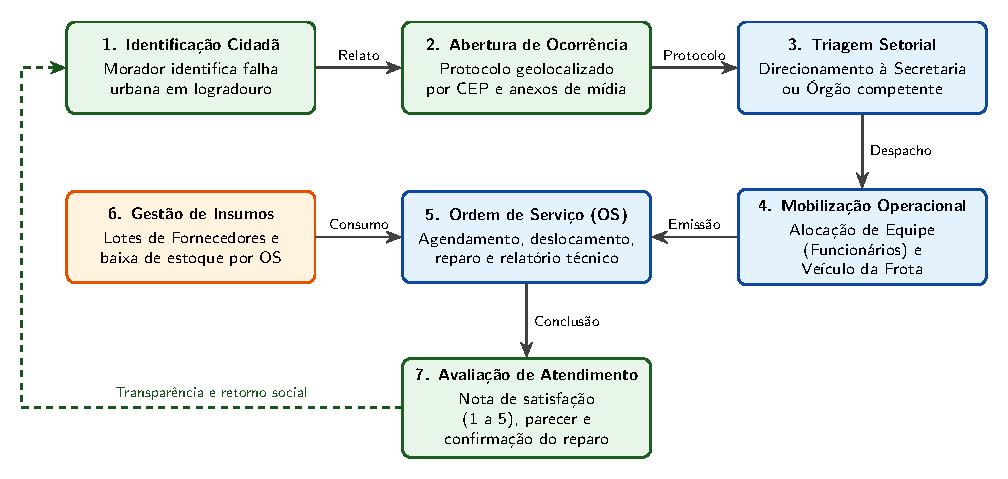
\includegraphics[width=0.95\textwidth]{figuras/fluxo-zeladoria.pdf}
\legend{Fonte: Elaborado pelos autores (2026).}
\end{figure}

\section{Causas Estruturais e Impactos Socioeconômicos, Ambientais e de Saúde}
\label{sec:causas-impactos}

As deficiências observadas decorrem de causas tecnológicas e organizacionais acumuladas na gestão pública local. Destaca-se a prevalência de sistemas departamentais isolados (\emph{silos de dados}), nos quais o registro de atendimento ao cidadão não se comunica com o controle de frotas, recursos humanos e almoxarifado \cite{ibge2024munic}, somada à ausência de padronização territorial por CEP e de indicadores de desempenho que orientem a manutenção preventiva.

Os impactos dessa desarticulação atingem múltiplas dimensões da vida coletiva. Na segurança viária e mobilidade, buracos e semáforos apagados elevam o índice de sinistros de trânsito e causam danos materiais à frota circulante. Na segurança pública e inclusão social, ruas com iluminação inoperante agravam a vulnerabilidade à violência noturna, restringindo a circulação de mulheres, idosos e trabalhadores \cite{ipea2019ods11, ibge2025entorno}. No campo ambiental e de saúde pública, o acúmulo de entulho favorece vetores de arboviroses (como a dengue) e, ao obstruir bocas de lobo, desencadeia alagamentos e exposição a doenças de veiculação hídrica \cite{snis2023drenagem, snis2023residuos}. Economicamente, a demora em executar pequenos reparos multiplica o custo final de reconstrução do pavimento e das galerias.

\section{Atores Envolvidos no Ecossistema de Manutenção Urbana}
\label{sec:atores-envolvidos}

O ecossistema de manutenção urbana congrega cinco grupos de atores que produzem, gerenciam ou utilizam os dados do domínio \cite{heuser2009projeto}: (i) o \textbf{cidadão (morador)}, que identifica a anomalia, abre a ocorrência geolocalizada por CEP com fotos ou vídeos e avalia a resolução após o reparo; (ii) as \textbf{secretarias e órgãos municipais}, que administram o orçamento mensal, coordenam equipes e mantêm a frota; (iii) as \textbf{equipes de manutenção e seus funcionários} (engenheiros, eletricistas, calceteiros), que executam as Ordens de Serviço em campo; (iv) os \textbf{gestores de almoxarifado e frota}, que controlam o estoque de insumos e a disponibilidade dos veículos; e (v) os \textbf{fornecedores terceirizados}, empresas contratadas que entregam lotes de materiais à prefeitura. A Tabela~\ref{tab:atores-sistema} resume o papel e as lacunas enfrentadas por cada ator.

\begin{table}[htb]
\ABNTEXfontereduzida
\caption{Atores envolvidos no ciclo de manutenção urbana, papéis informacionais e dificuldades enfrentadas no modelo tradicional}
\label{tab:atores-sistema}
\centering
\begin{tabular}{L{2.7cm} L{4.2cm} L{4.0cm} L{3.3cm}}
\toprule
\textbf{Ator} & \textbf{Papel no Processo} & \textbf{Dados Produzidos ou Utilizados} & \textbf{Principal Lacuna no Fluxo Tradicional} \\
\midrule
Cidadão (Morador) & Identifica falhas urbanas no território, abre ocorrências e audita o resultado do reparo & Cadastro pessoal, CEP de moradia, relato da ocorrência, mídias e avaliação de atendimento & Falta de retorno sobre o protocolo e impossibilidade de avaliar a solução \\
Secretarias e Órgãos Municipais & Coordenam equipes, gerenciam frota e controlam a execução do orçamento mensal da pasta & Dados da secretaria, orçamento mensal, indicadores de gravidade, custos de OS e avaliações & Visão fragmentada das demandas por bairro e dos gastos reais por reparo \\
Equipes e Funcionários de Campo & Deslocam-se aos locais das ocorrências e executam os reparos técnicos agendados & Turno, disponibilidade, matrícula, cargo, Ordem de Serviço, veículo alocado e relatório técnico & Endereços imprecisos em campo e falta de triagem prévia por imagem \\
Gestão de Almoxarifado e Frota & Controla o estoque de materiais e o estado de conservação dos veículos operacionais & Catálogo de insumos, saldo em estoque, custo médio, baixas por OS e status de veículos & Baixas manuais sem vínculo com a OS e risco de ruptura de estoque \\
Fornecedores Terceirizados & Suprem a prefeitura com insumos de manutenção por meio de lotes contratados & CNPJ, razão social, número de lote de compra, data de entrega, quantidade e preço unitário & Dificuldade de rastrear lotes entregues e variação histórica de preços \\
\bottomrule
\end{tabular}
\legend{Fonte: Elaborado pelos autores (2026).}
\end{table}

\section{Soluções Existentes, Marco Legal e Lacunas Persistentes}
\label{sec:solucoes-lacunas}

No Brasil, o dever estatal de manutenção urbana participativa ampara-se na Lei n\textsuperscript{o}~10.257/2001 (\emph{Estatuto da Cidade}) \cite{brasil2001estatutocidade}, que consagra a gestão democrática da cidade e o direito à infraestrutura urbana, e na Lei n\textsuperscript{o}~13.460/2017 (\emph{Código de Defesa dos Usuários dos Serviços Públicos}) \cite{brasil2017lei13460}, que exige o registro informatizado de manifestações e a avaliação continuada dos serviços públicos por indicadores de satisfação. Embora diversas prefeituras tenham adotado aplicativos do tipo ``156 digital'' \cite{ibge2024munic}, a maioria restringe-se à recepção de chamados (\emph{front-office}), sem modelar a operação de engenharia e suprimentos (\emph{back-office}): inexistem vínculos relacionais entre a ocorrência aberta pelo cidadão, a Ordem de Serviço executada, a equipe e o veículo mobilizados, os lotes de compra de fornecedores e a baixa individualizada de materiais consumidos no reparo.

\section{O Papel Estruturante de um Sistema de Banco de Dados Relacional}
\label{sec:papel-banco-dados}

A superação dessas lacunas requer um banco de dados relacional que assegure integridade referencial, controle de redundância e cruzamento estruturado de dados \cite{elmasri2019sistemas}. No domínio analisado, o banco de dados integra três eixos fundamentais: (i) a \textbf{padronização geográfica e cidadã}, vinculando moradores e ocorrências a uma base única de regiões de CEP e preservando os anexos de mídia comprobatória; (ii) a \textbf{gestão operacional interna}, relacionando secretarias, equipes de manutenção, funcionários e veículos da frota às Ordens de Serviço geradas para cada ocorrência; e (iii) a \textbf{rastreabilidade de insumos e auditoria social}, controlando os lotes de compra entregues por fornecedores, o consumo de materiais em cada Ordem de Serviço e a avaliação final de satisfação registrada pelo cidadão solicitante.
